\def\probtitle{안전한 건설 계획}
\def\probno{F}

\begin{problem}{\probno{}. \probtitle{}}

숭실대학교는 새로운 고층 건물을 설계하고 있다.

현재까지 쌓아 올린 건물의 골조는 수직 방향으로 세운 $N$개의 기둥, 그리고 서로 다른 두 기둥을 수평으로 연결하는 $M$개의 빔으로 구성되어 있다. 즉, 현재까지 쌓아 올린 건물 골조의 평면도는 아래 그림처럼 기둥을 점의 형태로, 빔을 점과 점을 연결하는 선분 형태로 나타낼 수 있다. 각 기둥은 $1$번부터 $N$번까지 번호가 붙어 있고 각 빔도 $1$번부터 $M$번까지 번호가 붙어 있다.

\begin{figure}[!h]
    \centering
    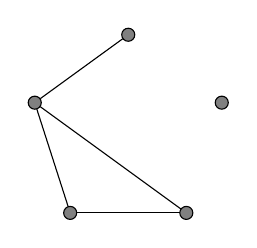
\begin{tikzpicture}[every node/.style={draw, fill=gray, scale=0.5}]
        \def \h {1.25}
        \node[circle] (1) at (0, 1*\h) {};
        \node[circle] (2) at (-0.95*\h, 0.31*\h) {};
        \node[circle] (3) at (0.95*\h, 0.31*\h) {};
        \node[circle] (4) at (-0.59*\h, -0.81*\h) {};
        \node[circle] (5) at (0.59*\h, -0.81*\h) {};
        \draw (1) -- (2);
        \draw (2) -- (4);
        \draw (2) -- (5);
        \draw (4) -- (5);
    \end{tikzpicture}
    \caption{5개의 기둥과 4개의 빔으로 구성된 골조}
\end{figure}


숭실대학교는 건물의 안정성을 강화하기 위해 몇 차례의 보강 작업을 진행해서 모든 서로 다른 두 기둥을 연결하는 빔이 존재하도록, 건물에 총 $N(N-1)/2$개의 빔을 설치하려고 한다. 즉, 기둥의 개수가 5개라고 하면 평면도가 아래 그림처럼 되도록 만들려고 한다.

\begin{figure}[!h]
    \centering
    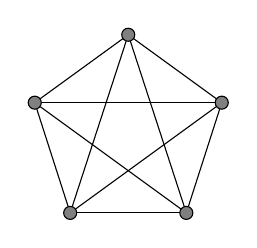
\begin{tikzpicture}[every node/.style={draw, fill=gray, scale=0.5}]
        \def \h {1.25}
        \node[circle] (1) at (0, 1*\h) {};
        \node[circle] (2) at (-0.95*\h, 0.31*\h) {};
        \node[circle] (3) at (0.95*\h, 0.31*\h) {};
        \node[circle] (4) at (-0.59*\h, -0.81*\h) {};
        \node[circle] (5) at (0.59*\h, -0.81*\h) {};
        \draw (1) -- (2);
        \draw (1) -- (3);
        \draw (1) -- (4);
        \draw (1) -- (5);
        \draw (2) -- (3);
        \draw (2) -- (4);
        \draw (2) -- (5);
        \draw (3) -- (4);
        \draw (3) -- (5);
        \draw (4) -- (5);
    \end{tikzpicture}
    \caption{5개의 기둥과 10개의 빔으로 구성된 골조}
\end{figure}

구조물의 하중을 지탱하기 위해, 보강 작업은 삼각형을 쌓아 나가는 방식으로 진행해야 한다. 구체적으로, 보강 작업은 서로 다른 세 기둥 $a, b, c$를 선택해서 $(a, b), (b, c), (c, a)$ 세 쌍을 모두 빔으로 연결하는 삼각형을 한 번에 쌓는 작업이다. 이때, 기존에 세 기둥 사이에 빔이 몇 개 있었는지에 따라 보강 작업에 필요한 비용이 달라진다.

\begin{figure}[h!]
\centering
    \begin{subfigure}[b]{.22\textwidth}
        \centering
        \begin{tikzpicture}[every node/.style={draw, fill=gray, scale=0.5}]
            \def \h {1.25}
            \node[circle] (1) at (0, 1.73*\h) {};
            \node[circle] (2) at (-1*\h, 0) {};
            \node[circle] (3) at (1*\h, 0) {};
        \end{tikzpicture}
        \caption{작업 진행 불가능}
    \end{subfigure}%
    \hfill
    \begin{subfigure}[b]{.22\textwidth}
        \centering
        \begin{tikzpicture}[every node/.style={draw, fill=gray, scale=0.5}]
            \def \h {1.25}
            \node[circle] (1) at (0, 1.73*\h) {};
            \node[circle] (2) at (-1*\h, 0) {};
            \node[circle] (3) at (1*\h, 0) {};
            \draw (1) -- (2);
        \end{tikzpicture}
        \caption{작업 비용 1}
    \end{subfigure}%
    \hfill
    \begin{subfigure}[b]{.22\textwidth}
        \centering
        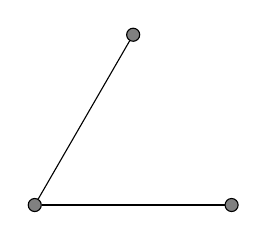
\begin{tikzpicture}[every node/.style={draw, fill=gray, scale=0.5}]
            \def \h {1.25}
            \node[circle] (1) at (0, 1.73*\h) {};
            \node[circle] (2) at (-1*\h, 0) {};
            \node[circle] (3) at (1*\h, 0) {};
            \draw (1) -- (2);
            \draw (2) -- (3);
        \end{tikzpicture}
        \caption{작업 비용 0}
    \end{subfigure}%
    \hfill
    \begin{subfigure}[b]{.22\textwidth}
        \centering
        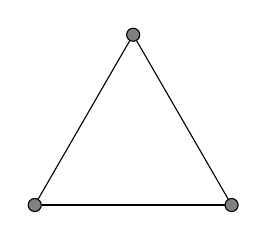
\begin{tikzpicture}[every node/.style={draw, fill=gray, scale=0.5}]
            \def \h {1.25}
            \node[circle] (1) at (0, 1.73*\h) {};
            \node[circle] (2) at (-1*\h, 0) {};
            \node[circle] (3) at (1*\h, 0) {};
            \draw (1) -- (2);
            \draw (2) -- (3);
            \draw (1) -- (3);
        \end{tikzpicture}
        \caption{작업 필요 없음}
    \end{subfigure}%
    \caption{빔 개수에 따른 보강 작업 비용}
\end{figure}

\begin{itemize}[noitemsep]
    \item 세 기둥 사이에 빔이 하나도 없는 경우: 작업의 위험도가 높으므로 진행할 수 없다.
    \item 세 기둥 사이에 1개의 빔이 있는 경우: 빔이 2개 추가되어 삼각형이 만들어지며, 이 작업에는 주의가 필요하므로 1만큼의 비용이 든다.
    \item 세 기둥 사이에 2개의 빔이 있는 경우: 빔이 1개 추가되어 삼각형이 만들어지며, 이 작업은 비교적 안전하므로 비용이 들지 않는다.
    \item 세 기둥 사이에 3개의 빔이 모두 있는 경우: 이미 삼각형이 구성되어 있으므로 아무것도 진행하지 않는다.
\end{itemize}

보강 작업을 0회 이상 원하는 만큼 진행해서, 모든 기둥 사이에 빔이 존재하도록 하는 최소 비용을 구하라. 모든 입력에 대해 서로 다른 두 기둥을 연결하는 빔이 항상 존재하도록 보강 작업을 진행할 수 있음이 보장된다.

\begin{figure}[!h]
    \centering
    \begin{tikzpicture}[every node/.style={draw, fill=gray, scale=0.5}]
        \def \h {1.25}
        \node[circle] (1) at (-1*\h, 1*\h) {};
        \node[circle] (2) at (1*\h, 1*\h) {};
        \node[circle] (3) at (1*\h, -1*\h) {};
        \node[circle] (4) at (-1*\h, -1*\h) {};
        \draw (1) -- (2);
        \draw (3) -- (4);
    \end{tikzpicture}
    \caption{예제 입력 1}
\end{figure}

예를 들어 골조의 평면도가 위 그림처럼 생겼고, 왼쪽 위에 있는 점부터 시계방향 순서대로 $1, 2, 3, 4$번 기둥이라고 해보자.

첫 번째 보강 작업에서 $1, 2, 3$번 기둥을 연결하는 삼각형을 만들고, 두 번째 보강 작업에서 $1, 2, 4$번 기둥을 연결하는 삼각형을 만들면 총합 $1+1=2$의 비용으로 완성할 수 있다.

반면, 첫 번째 보강 작업에서 $1, 2, 3$번 기둥, 두 번째 보강 작업에서 $2, 3, 4$번 기둥, 세 번째 보강 작업에서 $1, 2, 4$번 기둥을 선택하면 총합 $1+0+0=1$의 비용으로 완성할 수 있다.

\begin{figure}[h!]
\centering
    \begin{subfigure}[b]{.22\textwidth}
        \centering
        \begin{tikzpicture}[every node/.style={draw, fill=gray, scale=0.5}]
            \def \h {1.25}
            \node[circle] (1) at (-1*\h, 1*\h) {};
            \node[circle] (2) at (1*\h, 1*\h) {};
            \node[circle] (3) at (1*\h, -1*\h) {};
            \node[circle] (4) at (-1*\h, -1*\h) {};
            \draw (1) -- (2);
            \draw (3) -- (4);
        \end{tikzpicture}
        \caption{작업 진행 전}
    \end{subfigure}%
    \hfill
    \begin{subfigure}[b]{.22\textwidth}
        \centering
        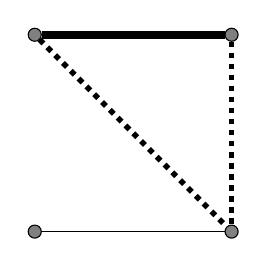
\begin{tikzpicture}[every node/.style={draw, fill=gray, scale=0.5}]
            \def \h {1.25}
            \node[circle] (1) at (-1*\h, 1*\h) {};
            \node[circle] (2) at (1*\h, 1*\h) {};
            \node[circle] (3) at (1*\h, -1*\h) {};
            \node[circle] (4) at (-1*\h, -1*\h) {};
            \draw[line width=1.0mm] (1) -- (2);
            \draw[dotted,line width=0.7mm] (1) -- (3);
            \draw[dotted,line width=0.7mm] (2) -- (3);
            % \draw[line width=0.7mm,draw=blue] (1) -- (2);
            % \draw[dotted,line width=0.7mm,draw=red] (1) -- (3);
            % \draw[dotted,line width=0.7mm,draw=red] (2) -- (3);
            \draw (3) -- (4);
        \end{tikzpicture}
        \caption{첫 번째 작업 후}
    \end{subfigure}%
    \hfill
    \begin{subfigure}[b]{.22\textwidth}
        \centering
        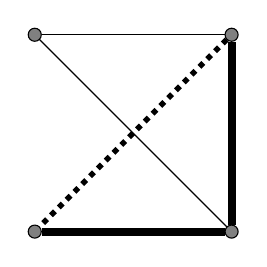
\begin{tikzpicture}[every node/.style={draw, fill=gray, scale=0.5}]
            \def \h {1.25}
            \node[circle] (1) at (-1*\h, 1*\h) {};
            \node[circle] (2) at (1*\h, 1*\h) {};
            \node[circle] (3) at (1*\h, -1*\h) {};
            \node[circle] (4) at (-1*\h, -1*\h) {};
            \draw (1) -- (2);
            \draw (1) -- (3);
            \draw[line width=1.0mm] (2) -- (3);
            \draw[dotted,line width=0.7mm] (2) -- (4);
            \draw[line width=1.0mm] (3) -- (4);
            % \draw[line width=0.7mm,draw=blue] (2) -- (3);
            % \draw[dotted,line width=0.7mm,draw=red] (2) -- (4);
            % \draw[line width=0.7mm,draw=blue] (3) -- (4);
        \end{tikzpicture}
        \caption{두 번째 작업 후}
    \end{subfigure}%
    \hfill
    \begin{subfigure}[b]{.22\textwidth}
        \centering
        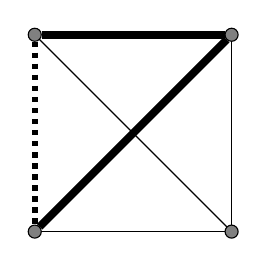
\begin{tikzpicture}[every node/.style={draw, fill=gray, scale=0.5}]
            \def \h {1.25}
            \node[circle] (1) at (-1*\h, 1*\h) {};
            \node[circle] (2) at (1*\h, 1*\h) {};
            \node[circle] (3) at (1*\h, -1*\h) {};
            \node[circle] (4) at (-1*\h, -1*\h) {};
            \draw (1) -- (3);
            \draw (2) -- (3);
            \draw (3) -- (4);
            \draw[line width=1.0mm] (1) -- (2);
            \draw[dotted,line width=0.7mm] (1) -- (4);
            \draw[line width=1.0mm] (2) -- (4);
            % \draw[line width=0.7mm,draw=blue] (1) -- (2);
            % \draw[dotted,line width=0.7mm,draw=red] (1) -- (4);
            % \draw[line width=0.7mm,draw=blue] (2) -- (4);
        \end{tikzpicture}
        \caption{세 번째 작업 후}
    \end{subfigure}%
    \caption{예제 출력 1}
\end{figure}

이 밖에도 여러 방법이 있지만, 비용을 $1$보다 적게 사용하는 방법은 없으므로 $1$이 최소 비용이다.

\InputFile

첫째 줄에 건물의 골조를 구성하는 기둥의 개수 $N$과 빔의 개수 $M$이 공백으로 구분되어 주어진다.

둘째 줄부터 $M+1$번째 줄까지, $i+1$번째 줄에 $i$번째 빔이 연결하는 두 기둥의 번호 $a_i, b_i$가 공백으로 구분되어 주어진다.

\OutputFile

보강 작업을 최적으로 진행할 때, 모든 서로 다른 기둥을 연결하는 빔이 존재하도록 만드는 최소 비용을 출력한다.

\Constraints

\begin{itemize}[noitemsep]
    \item $3 \leq N \leq 40$
    \item $1 \leq M \leq N(N-1)/2$
    \item $1 \leq a_i < b_i \leq N$ $(1 \le i \le M)$ 
    \item $i \neq j$ 이면 $(a_i, b_i) \neq (a_j, b_j)$이다. $(1 \le i, j \le M)$ 즉, 연결하는 두 기둥의 쌍이 동일한 빔이 여러 개 존재하지 않는다.
    \item 서로 다른 두 기둥을 연결하는 빔이 항상 존재하도록 보강 작업을 진행할 수 있음이 보장된다.
    \item 입력으로 주어지는 수는 모두 정수이다.
\end{itemize}

\Example

\begin{example}
    \exmpfile{./example/01.in.txt}{./example/01.out.txt}%
    \exmpfile{./example/02.in.txt}{./example/02.out.txt}%
    \exmpfile{./example/03.in.txt}{./example/03.out.txt}%
\end{example}

세 번째 예시는 첫 번째 보강 작업에서 $1, 2, 3$번 기둥, 두 번째 보강 작업에서 $1, 3, 4$번 기둥, 세 번째 보강 작업에서 $1, 2, 4$번 기둥을 선택하면 $0$만큼의 비용이 든다.

% \newpage

% \Notes


\end{problem}